
\section{Experimental set up to obtain profile views of the droplet}

\par To create a heater, cartridge resistance heaters were put under an aluminum plate, radiating to its surface. The experiment was made for water droplets impacts on a hydrophilic silicon wafer surface \\

\par In the interface of the silicon wafer and the aluminum plate a thermal paste was used to improve heat transfer. On top of the silicon wafer there is a thermocouple that monitors the surface temperature. This setup can be seen in detail in Figure \ref{fig:horizontal2}. The thermocouple value is used by a PID controller to control the heat released by the cartridge heater.\\

\begin{figure}[h]
\centering
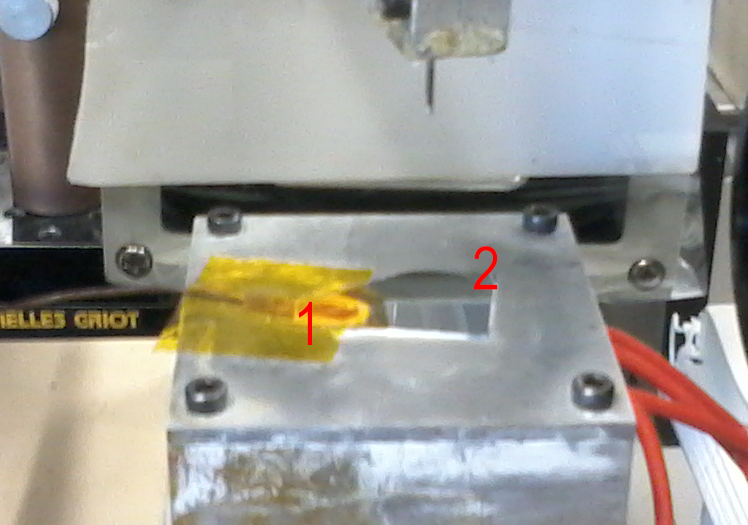
\includegraphics[width=0.5\linewidth]{Figures/3.Chapter/horizontal2.png}
\caption{Silicon Wafer setup: (1) Thermocouple, (2) Silicon Wafer}
\label{fig:horizontal2}
\end{figure}

\par An Harvard Apparatus controls a syringe's water discharge, that then falls from the needle to the wafer. This forms a droplet with 2.6 to 3 mm diameter spherical droplet. This experiment is recorded by 2 cameras: IR camera and high-speed camera. In order for the high-speed camera to work, a high intensity lamp is also needed. The described setting can be seen in Figure \ref{fig:horizontal}. This setting was used to gather qualitative results only. Good quantitative results are impossible due to the implications of droplet geometry in thermography. The images taken by the high speed camera were recorded at 2200 fps. The calibration factor used was 26 px/mm. The calibration factor for the IR camera was 6 px/mm.

\begin{figure}[h]
\centering
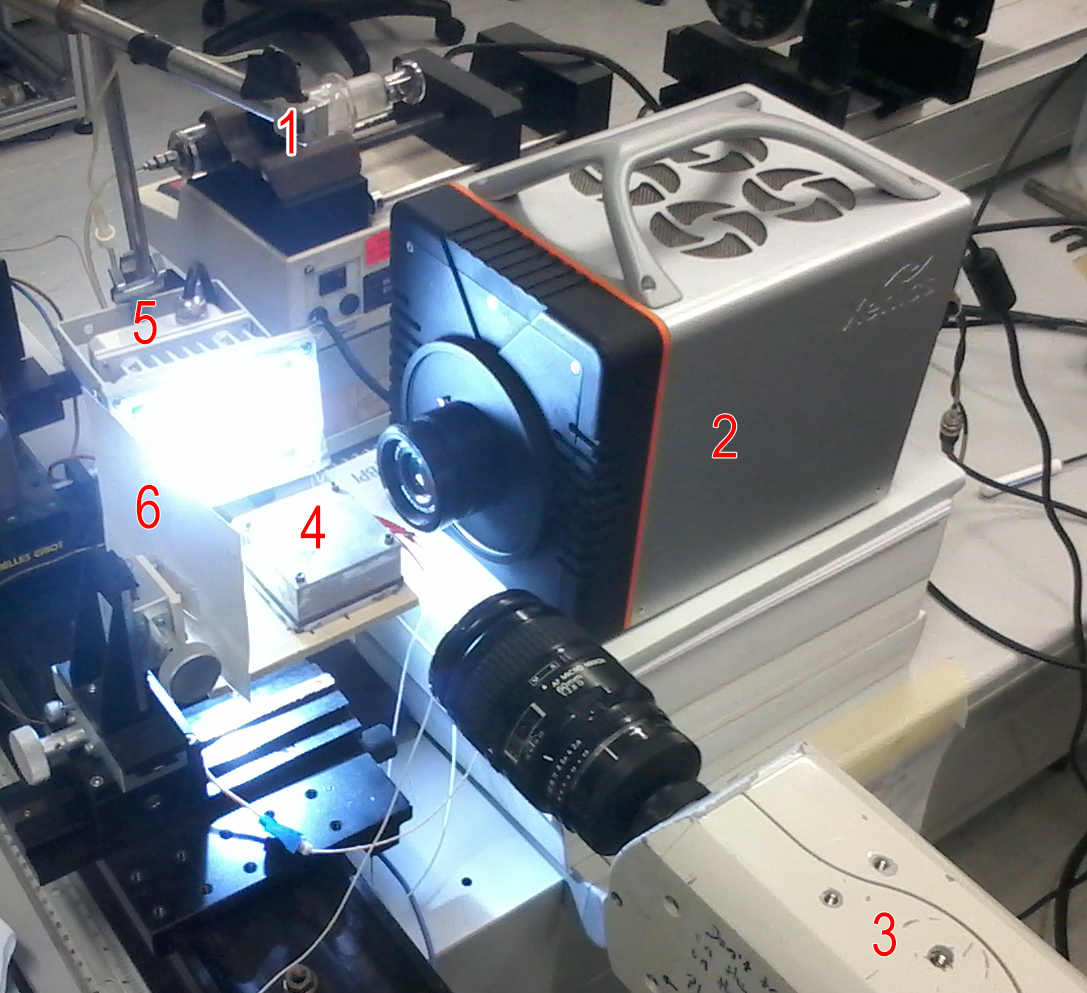
\includegraphics[width=0.65\linewidth]{Figures/3.Chapter/horizontal.png}
\caption{Horizontal setup: (1) Needle, (2) IR Camera, (3) HS Camera, (4) Heated Surface, (5) Lamp, (6) Black Background}
\label{fig:horizontal}
\end{figure}

\subsection{Procedure}
\label{sec:procedure}
\begin{itemize}
\item Adjust IR Camera's settings on the software.
\item Perform an offset calibration (described in Section \ref{sec:icam}).
\item Adjust PID controller to the desired temperature and water flow in the Harvard Apparatus.
\item Set the cameras recording.
\item Let a droplet fall on the wafer.
\item Clean the wafer with acetone and distilled water before proceeding to a new test.
\end{itemize}

\section{Bottom View of the metal foil}

\par In this setup, the IR Camera is placed underneath the surface on which the droplet impacts. The droplet impacts on a 20 $\mu m$ thick stainless steel foil. This was done similarly to \cite{sielaff2014experimental}, as the objective was to read the interface temperatures. Due to of the small thickness of the foil, the temperature of the interface is very similar to the read temperature in the bottom of the foil. The HS camera was placed horizontally to the foil to observe the impact. A lamp was placed in the opposite side. The setup scheme can be seen in Figure \ref{fig:setup}.\\

\begin{table}[h]
\centering
\caption{Thermophysical Properties of the Studied Liquids}
\label{tab:props}
\begin{tabular}{lcc}
\toprule
\multicolumn{1}{c}{Characteristics} & \multicolumn{1}{c}{Water} & \multicolumn{1}{c}{Ethanol} \\
\cmidrule[0.4pt](r{0.125em}){1-3}%
Saturation Temperature ($T_{sat}[ºC]$)       & 100                 & 78.3         \\
Density ($\rho[kg/m^3]$)                   & 1000                & 757          \\
Kinematic Viscosity ($\mu[10^{-3}Ns/m^2]$) & 1.05                & 1.19         \\
Surface Tension ($\sigma[10^{-3}N/m]$)     & 72.88               & 22.8         \\ \bottomrule
\end{tabular}
\end{table}

\begin{figure}[h]
\centering
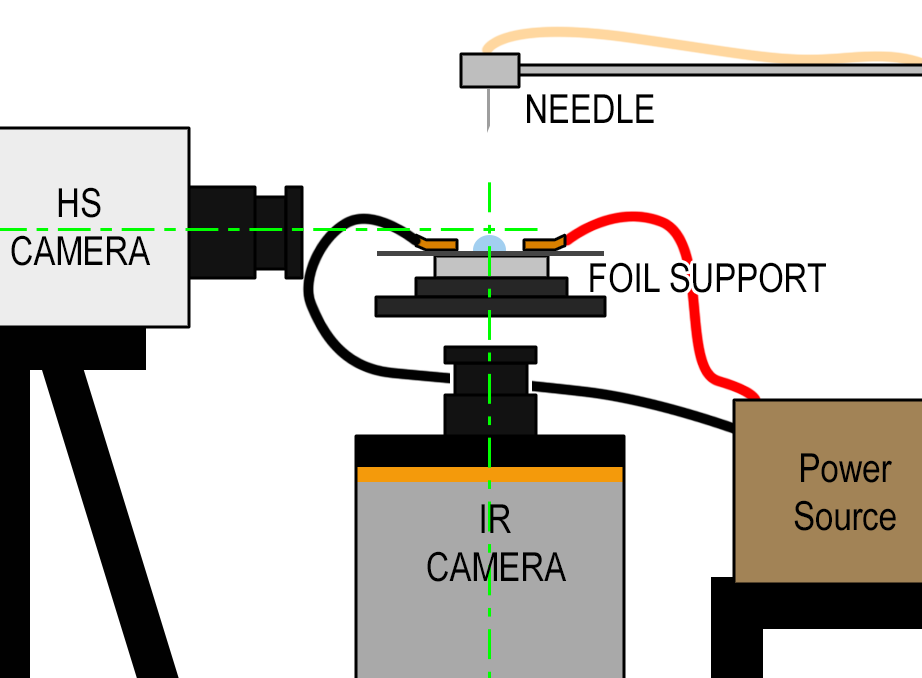
\includegraphics[width=0.55\linewidth]{Figures/3.Chapter/setup.png}
\caption{Bottom Setup Scheme}
\label{fig:setup}
\end{figure}

\par The experiments performed using this setup were made using hydrophilic (using distilled water and ethanol) and super-hydrophobic (using just water) surfaces. A preliminary experiment with water and an hydrophilic surface was made, using the software calibration. From the first, raw results were taken for posterior calibration and processing. The calibrations and their differences are explained in Chapter \ref{cap:setup}. Table \ref{tab:props} summarizes the main physical properties of the working fluids \cite{tfc}.\\

\par The foil is fed by an electric current, so it can heat up to the desired temperature. This is done by to electrical contacts, wired to a power source. The foil has to be placed on top of a bad heat conductor to minimize heat losses. A heat glass was chosen for the purpose. The foil must be stretched so that possible wrinkles don't affect the droplet motion. A detail of the setup, on the foil support can be seen in Figure \ref{fig:suporte}. In this figure two supports are shown. The second was made after the calibration. \\

\par To prepare the super-hydrophobic surfaces, the surfaces needed to be cleaned with an ultra-sound bath and coated with \textit{Glaco}\textregistered \cite{kato2011durable}. This coating took several layers to ensure effective coating that can endure high temperature and droplet impacts. \\

\begin{figure}[h]
\centering
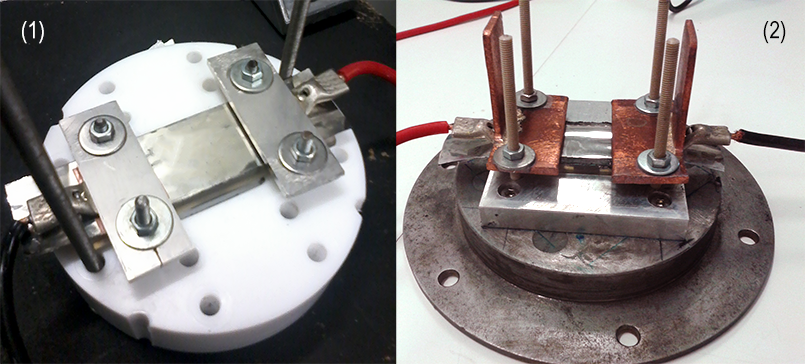
\includegraphics[width=0.9\linewidth]{Figures/3.Chapter/suporte.png}
\caption{Stainless Steel Support: (1) Before calibration setup, (2) After calibration setup}
\label{fig:suporte}
\end{figure}

\par This setup also was the Harvard Apparatus and the needle to generate the droplet. A metal structure holds the support, needle and the camera. The complete setup can be seen in Figure \ref{fig:setup2}. Although one have a different calibration, the procedure is similar to the previously described in \ref{sec:procedure}. The big difference is that the foil temperature is controlled with the power source and not with the PID. To adjust the current correctly one needs to read the temperature on the IR Camera's software. In the case that raw images are needed, an additional step should be to convert the desired temperatures in ADU. Only this procedure allows knowing if the foil is at the desired temperature.

\begin{figure}[h]
\centering
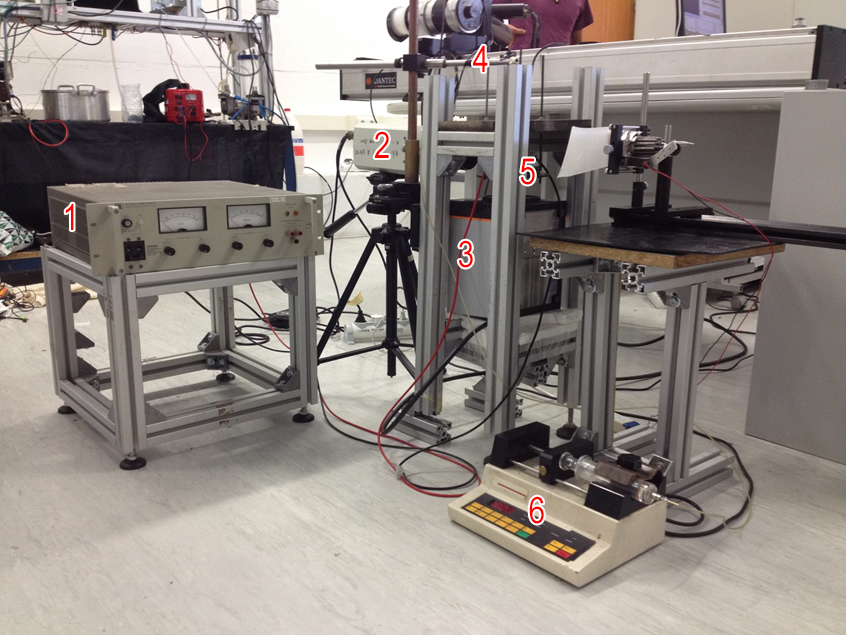
\includegraphics[width=0.9\linewidth]{Figures/3.Chapter/setup2.png}
\caption{Bottom Setup: (1) Power Source, (2) HS Camera, (3) IR Camera, (4) Needle, (5) Foil Support, (6) Harvard Apparatus}
\label{fig:setup2}
\end{figure}

\section{Surface preparation and Characterization}
\par The stainless steel foils (coated and uncoated) were characterized in terms of surface topography and wettability. Surface topography was measured a profile meter (Dektak 3 - Veeco) with a vertical resolution of 20 nm. The foil was found to be smooth within this resolution. The wettability was characterized measuring the contact angle with an optical profile meter (THETA from Attention) using the droplet method, as described for instance in Moita \textit{et. al.} (2016) \cite{moita2016dynamics}. The contact angle values are taken as an average of 5 measurements performed at different regimes of the surfaces. The contact angle is $\theta = 87.05º$ for the hydrophilic surface and $\theta = 162.47º$ for the super-hydrophobic surface.\\
\par Hysterisis, evaluated also as in Moita \textit{et. al.} (2016) \cite{moita2016dynamics} was found to be lower than 10º for the surface with the highest contact angle (coated with \textit{Glaco}\textregistered) thus confirming its super-hydrophobic nature.